%!TEX program = xelatex
\documentclass[11pt, a4paper]{article}
  \usepackage[a4paper,top=3cm,bottom=4cm,left=2.5cm,right=2.5cm]{geometry}
  \usepackage{subfig}
  \usepackage{graphicx}
  \graphicspath{{../images/}}
  \usepackage{hyperref}
  \usepackage{amsmath}
  \usepackage{braket}
  \usepackage{enumitem}
  \usepackage{multirow}
  \usepackage{mathtools}
  \usepackage{xepersian}
  \settextfont[Scale=1.2]{B Nazanin}
  \setlatintextfont[Scale=1]{Times New Roman Cyr}
  \title{\textbf{شبیه‌سازی رایانه‌ای در فیزیک}\\تمرین نهم: دینامیک مولکولی}
  \author{سینا معمر ۹۵۱۰۲۳۱۶}
    

\begin{document}

\maketitle
\thispagestyle{empty}


\section{\textbf{مدل دینامیک مولکولی}}
کد این بخش از تمرین را در فایل
\lr{md.py}
می توان مشاهده نمود.
در این فایل دو کلاس
\lr{SingleAtomMD}
و
\lr{DataAnalysis}
وجود دارد که هر یک در ادامه توضیح داده خواهند شد.
\\
برای ایجاد یک مدل دینامیک مولکولی برای ذرات تک اتمی،
باید یک
\lr{object}
از کلاس
\lr{SingleAtomMD}
با طول جعبه، تعداد ذرات، بعد مسئله و اطلاعات اتمی مربوط به آن ‌ذره دل‌خواه بسازیم.
با توجه به خواسته‌ی تمرین، با استفاده از تابع
\lr{\_place\_atoms\_left\_side\_regularly}
ذرات در لحظه‌ی اولیه به طور منظم در نیمه‌ی چپ جعبه قرار می‌گیرند.
سپس با فراخوانی تابع
\lr{\_periodic\_boundaries}
شرایط مرزی تناوبی را اعمال می‌کنیم.
با توجه به حداکثر سرعت داده شده، سرعت اولیه ذرات را با استفاده از تابع
\lr{\_assign\_initial\_velocities}
تعیین می‌کنیم.
به گونه‌ای که همگی سرعت یکسان ولی در جهات تصادفی خواهند داشت.
برای به دست آوردن ماتریس فاصله‌ها نیز تابع
\lr{\_update\_positions\_diff}
را باید فراخوانی کنیم.
هم‌چنین با استفاده از تابع
\lr{\_update\_distance\_matrices}
ماتریس اندازه‌ی فواصل ذرات در توان‌های
$-2$،
$-6$
و
$-12$
را محاسبه می‌کنیم.
در نهایت نیز شتاب ذرات را با تابع
\lr{\_update\_accelerators}
به دست می‌آوریم.
اکنون مدل ما آماده اجرا شده و با استفاده از تابع
\lr{\_initialize\_files}
فایل‌های ذخیره‌سازی و اطلاعات مدل را آماده می‌کنیم.


\section{\textbf{شبیه‌سازی ۱۰۰ ذره}}
برای شبیه‌سازی با توجه به خواسته‌ی سوال، یک
\lr{object}
از کلاس
\lr{SingleAtomMD}
با
$100$
ذره آرگون در یک جعبه‌ی دو بعدی به طول
$30$
می‌سازیم.
لازم به توجه است که تمام اعداد ذکر شده در متن، در واحد‌های کاهیده هستند.
سرعت اولیه‌ی ذرات را
$1.5$
و طول قدم‌های انتگرال‌گیری‌مان را
$10^{-3}$
در نظر می‌گیریم.
شبیه‌سازی را با استفاده از تابع
\lr{render}
و برای
$200\,000$
قدم یا معادلا به اندازه‌ی
$200$
واحد زمانی می‌گذاریم انجام بشود و در هر
$100$
قدم نیز از سیستم نمونه‌گیری می‌کنیم.


\subsection{بقای انرژی سیستم}
برای بررسی بقای انرژی سیستم نمودار انرژی‌های جنبشی، پتانسیل و انرژی کل را در یک نمودار رسم می کنیم.
نمودار به دست آمده را در شکل
\ref{fig:100_energies}
می‌توان مشاهده نمود.
همان‌طور که دیده می‌شود با وجود نوسانات انرژی جنبشی و پتانسیل در طول شبیه‌سازی،
مقدار انرژی کل تغییری نکرده و ثابت باقی می ماند.
این ثابت بودن به علت استفاده از الگوریتم ورله سرعتی در انتگرال‌گیری‌‌مان در شبیه‌سازی و استفاده از طول قدم مناسب است.

\begin{figure}[h!]
	\centering
  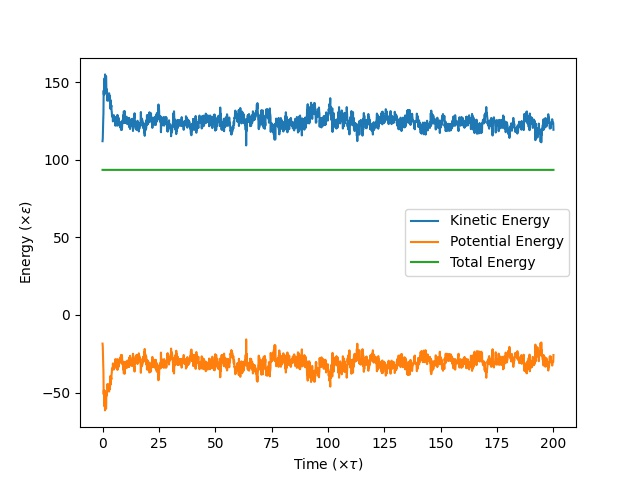
\includegraphics[width=.7\textwidth]{MD_30_100_2_0.001_energies.jpg}
  \caption{تغییرات انرژی جنبشی، پتانسیل و انرژی کل بر حسب زمان شبیه‌سازی برای $100$ ذره‌ی آرگون در جعبه‌ای به طول $30$ و با سرعت اولیه‌ی $1.5$}
  \label{fig:100_energies}
\end{figure}

\subsection{تعداد ذرات موجود در نیمه‌ی چپ}
یکی از روش ‌های نسبتا قابل قبول برای تعیین زمان رسیدن به تعادل شبیه‌سازی،
استفاده از تعداد ذرات موجود در نیمه‌ی چپ جعبه است.
می دانیم که در حالت تعادل این تعداد حول نصف ذرات باید نوسان کند.
نمودار به دست آمده را در شکل
\ref{fig:100_left_side}
می توان مشاهده نمود.
همان‌طور که دیده می‌شود این تعداد در حدود زمانی
$10$
به نصف مقدار می‌رسد و حول آن شروع به نوسان می‌کند.

\begin{figure}[h!]
	\centering
  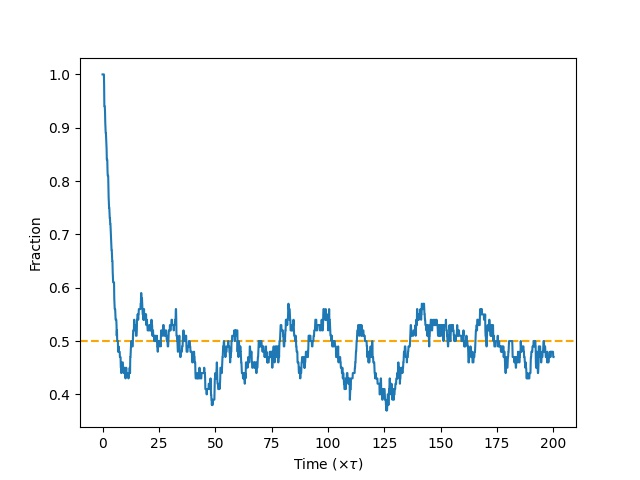
\includegraphics[width=.7\textwidth]{MD_30_100_2_0.001_left_side_numbers.jpg}
  \caption{تغییرات نسبت ذرات موجود در نیمه‌ی چپ جعبه بر حسب زمان شبیه‌سازی برای $100$ ذره‌ی آرگون در جعبه‌ای به طول $30$ و با سرعت اولیه‌ی $1.5$}
  \label{fig:100_left_side}
\end{figure}


\subsection{دمای گاز}
رفتار دما کاملا مشابه با رفتار انرژی جنبشی است. تنها اسکیل آن‌ها متفاوت می‌باشد.
نمودار به دست آمده را در شکل
\ref{fig:100_temperature}
می توان مشاهده نمود.
همان‌طور که دیده می‌شود دما در حدود زمان
$10$
به تعادل می رسد و حول آن نوسان می کند.
از آن‌جایی که تعداد ذرات ما کم است، دامنه‌ی این نوسانات به نسبت زیاد می‌باشد.
با میان‌گیری زمانی مقدار تعادلی آن برابر می‌شود با:
\begin{equation}
  \braket{T} = 1.257 \pm 0.001 \ (\times \epsilon / k_B) = 150.5 \pm 0.1 K
\end{equation}

\begin{figure}[h!]
	\centering
  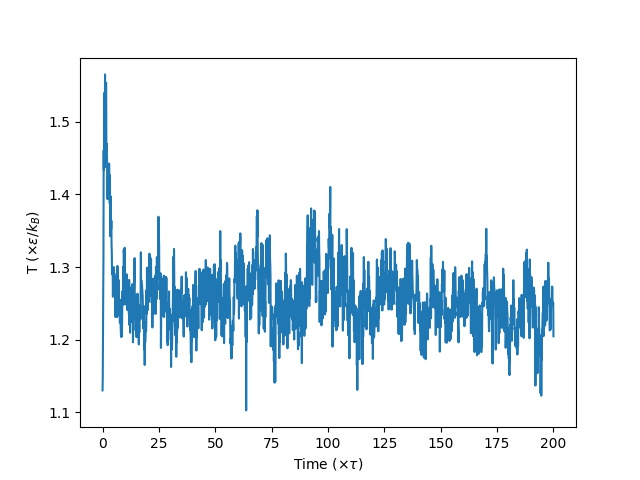
\includegraphics[width=.7\textwidth]{MD_30_100_2_0.001_temperatures.jpg}
  \caption{تغییرات دما بر حسب زمان شبیه‌سازی برای $100$ ذره‌ی آرگون در جعبه‌ای به طول $30$ و با سرعت اولیه‌ی $1.5$}
  \label{fig:100_temperature}
\end{figure}


\subsection{فشار گاز}
نمودار به دست آمده را در شکل
\ref{fig:100_pressure}
می توان مشاهده نمود.
همان‌طور که دیده می‌شود فشار در حدود زمان
$10$
به تعادل می رسد و حول آن نوسان می کند.
از آن‌جایی که تعداد ذرات ما کم است، دامنه‌ی این نوسانات به نسبت زیاد می‌باشد.
با میان‌گیری زمانی مقدار تعادلی آن برابر می‌شود با:
\begin{equation}
  \braket{P} = 0.143 \pm 0.001 \ (\times \epsilon / \sigma^2) = (2.0431 \pm 0.0001) \times 10^{-3} N/m
\end{equation}

\begin{figure}[h!]
	\centering
  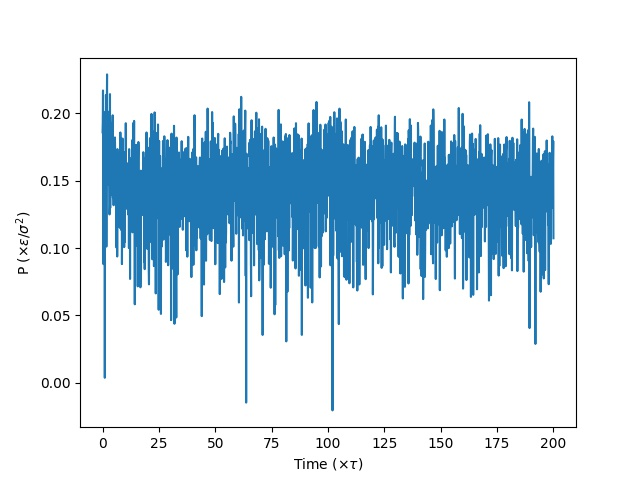
\includegraphics[width=.7\textwidth]{MD_30_100_2_0.001_pressures.jpg}
  \caption{تغییرات فشار بر حسب زمان شبیه‌سازی برای $100$ ذره‌ی آرگون در جعبه‌ای به طول $30$ و با سرعت اولیه‌ی $1.5$}
  \label{fig:100_pressure}
\end{figure}


\subsection{خودهم‌بستگی سرعت‌ها و زمان واهلش}
زمان واهلش، زمان مشخصه‌ی تابع خود‌هم‌بستگی سرعت‌ها است.
این زمان در واقع به ما نشان می دهد که چقدر زمان باید بگذرد تا سرعت‌های سیستم مقادیر اولیه خود را فراموش کنند.
نمودار به دست آمده را در شکل
\ref{fig:100_c_v}
می توان مشاهده نمود.
با توجه به نمودار به دست آمده، زمان واهلش برابر خواهد بود با:
\begin{equation}
  \tau = 1.9 (\times \tau)
\end{equation}

\begin{figure}[h!]
	\centering
  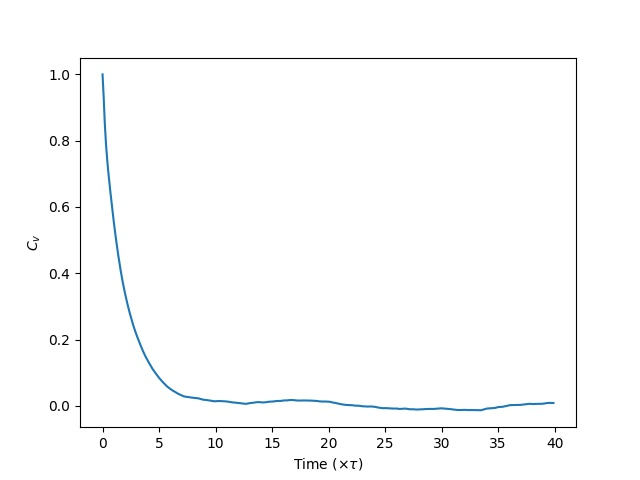
\includegraphics[width=.7\textwidth]{MD_30_100_2_0.001_c_v.jpg}
  \caption{تابع خود‌هم‌بستگی سرعت‌ها برای $100$ ذره‌ی آرگون در جعبه‌ای به طول $30$ و با سرعت اولیه‌ی $1.5$}
  \label{fig:100_c_v}
\end{figure}


\subsection{رابطه‌ی فشار با دما}
برای مشاهده‌ی رابطه‌ی فشار با دما،
مدل‌مان را برای اندازه‌ی سرعت اولیه‌‌های متفاوت اجرا می‌کنیم و مقادیر تعادلی دما و فشار را به دست می‌آوریم.
برای مثال در این قسمت، مقادیر دما و فشار را برای اندازه‌‌ی سرعت‌های
$1$
تا
$2$
با قدم‌هایی به طول
$0.05$
به دست می‌‌آوریم.
نمودار به دست آمده را در شکل
\ref{fig:100_P_T}
می توان مشاهده نمود.
همان‌طور که مشاهده می‌شود رابطه‌‌ای خطی میان فشار و دما وجود دارد.
که این مطابق با انتظار ما از معادله‌ی گاز واندروالس است.
معادله‌ی خط فیت شده برابر است با:
\begin{equation}
  P = 0.089T + 0.032
\end{equation}

\begin{figure}[h!]
	\centering
  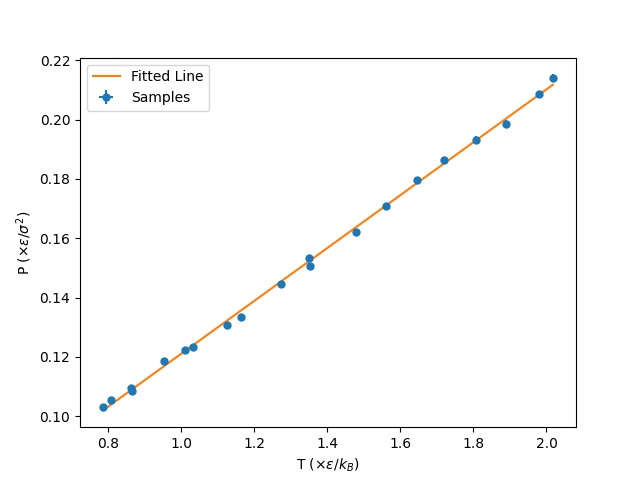
\includegraphics[width=.7\textwidth]{MD_30_100_2_0.001_P_T.jpg}
  \caption{تغییرات فشار بر حسب دما برای $100$ ذره‌ی آرگون در جعبه‌ای به طول $30$}
  \label{fig:100_P_T}
\end{figure}


\subsection{تغییر فاز سیستم}
برای مشاهده‌ی تغییر فاز سیستم باید نمودار انرژی بر حسب دما را برای مدل‌مان به دست بیاوریم.
در دماهایی که شیب تغییرات انرژی زیاد می‌شود و گویی جهش انرژی داریم، تغییر فاز رخ می‌دهد.
برای این‌ کار می‌گذاریم که شبیه‌سازی‌مان در یک دمای نسبتا زیاد به تعادل برسد.
سپس یک شبیه‌سازی دیگر با مکان‌ها و سرعت‌های شبیه‌سازی قبلی ایجاد می کنیم
با این تفاوت که سرعت‌ها را هر بار در یک ضریب کوچک‌تر از یک ضرب می کنیم.
به این ترتیب دمای سیستم را کاهش می دهیم و دما و انرژی تعادلی را به دست می‌آوریم.
نمودار به دست آمده را در شکل
\ref{fig:100_E_T}
می توان مشاهده نمود.
همان‌طور که مشاهده می‌شود، در حدود دمای
$0.6 (\times \epsilon / k_B)$
تا
$0.2 (\times \epsilon / k_B)$
شاهد تغییرات شدید انرژی در دو نقطه هستیم.
که این به آن معنی است که ظرفیت گرمایی بسیار بزرگی خواهیم داشت و تغییر فاز رخ می‌دهد.
\\
هم‌چنین این تفاوت رفتار گاز در این دو فاز را می توان در حرکت اتم‌ها نسبت به یکدیگر مشاهده کرد.
به همین دلیل از حرکت اتم‌ها در بالاترین دما و پایین‌ترین دما انیمیشن تهیه می‌سازیم.
این انیمیشن‌ها را در فایل
\lr{animations}
به اسم‌های
\lr{MD\_30 \_100\_2\_0.001\_gas\_phase.mp4}،
\lr{MD\_30 \_100\_2\_0.001\_liquid\_phase.mp4}
و
\lr{MD\_30 \_100\_2\_0.001\_solid\_phase.mp4}
می‌توان مشاهده نمود.

\begin{figure}[h!]
	\centering
  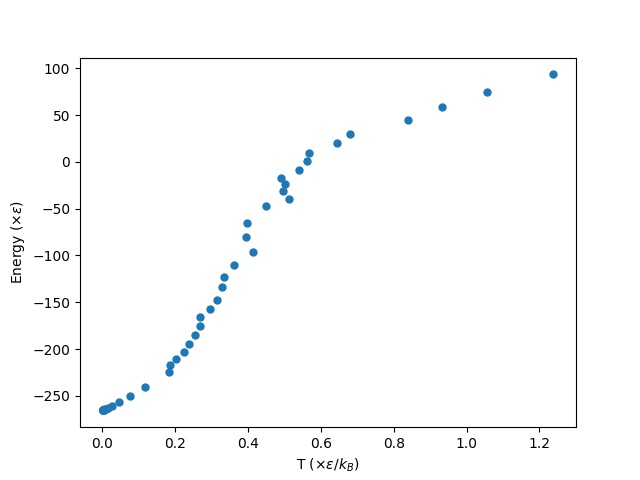
\includegraphics[width=.7\textwidth]{MD_30_100_2_0.001_E_T.jpg}
  \caption{تغییرات انرژی بر حسب دما برای $100$ ذره‌ی آرگون در جعبه‌ای به طول $30$}
  \label{fig:100_E_T}
\end{figure}


\section{\textbf{شبیه‌سازی ۱۰۰۰ ذره}}
برای شبیه‌سازی با توجه به خواسته‌ی سوال، یک
\lr{object}
از کلاس
\lr{SingleAtomMD}
با
$1000$
ذره آرگون در یک جعبه‌ی دو بعدی به طول
$90$
می‌سازیم.
لازم به توجه است که تمام اعداد ذکر شده در متن، در واحد‌های کاهیده هستند.
سرعت اولیه‌ی ذرات را
$1.5$
و طول قدم‌های انتگرال‌گیری‌مان را
$10^{-3}$
در نظر می‌گیریم.
شبیه‌سازی را با استفاده از تابع
\lr{render}
و برای
$100\,000$
قدم یا معادلا به اندازه‌ی
$100$
واحد زمانی می‌گذاریم انجام بشود و در هر
$100$
قدم نیز از سیستم نمونه‌گیری می‌کنیم.


\subsection{بقای انرژی سیستم}
برای بررسی بقای انرژی سیستم نمودار انرژی‌های جنبشی، پتانسیل و انرژی کل را در یک نمودار رسم می کنیم.
نمودار به دست آمده را در شکل
\ref{fig:1000_energies}
می‌توان مشاهده نمود.
همان‌طور که دیده می‌شود با وجود نوسانات انرژی جنبشی و پتانسیل در طول شبیه‌سازی،
مقدار انرژی کل تغییری نکرده و ثابت باقی می ماند.
این ثابت بودن به علت استفاده از الگوریتم ورله سرعتی در انتگرال‌گیری‌‌مان در شبیه‌سازی و استفاده از طول قدم مناسب است.

\begin{figure}[h!]
	\centering
  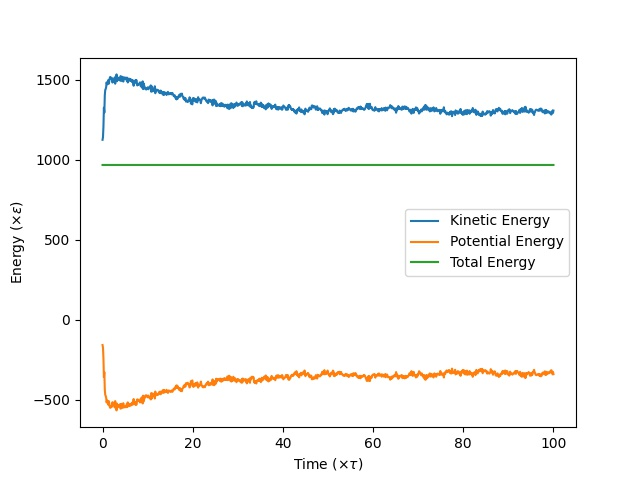
\includegraphics[width=.7\textwidth]{MD_90_1000_2_0.001_energies.jpg}
  \caption{تغییرات انرژی جنبشی، پتانسیل و انرژی کل بر حسب زمان شبیه‌سازی برای $1000$ ذره‌ی آرگون در جعبه‌ای به طول $90$ و با سرعت اولیه‌ی $1.5$}
  \label{fig:1000_energies}
\end{figure}

\subsection{تعداد ذرات موجود در نیمه‌ی چپ}
یکی از روش ‌های نسبتا قابل قبول برای تعیین زمان رسیدن به تعادل شبیه‌سازی،
استفاده از تعداد ذرات موجود در نیمه‌ی چپ جعبه است.
می دانیم که در حالت تعادل این تعداد حول نصف ذرات باید نوسان کند.
نمودار به دست آمده را در شکل
\ref{fig:1000_left_side}
می توان مشاهده نمود.
همان‌طور که دیده می‌شود این تعداد در حدود زمانی
$30$
به نصف مقدار می‌رسد و حول آن شروع به نوسان می‌کند.

\begin{figure}[h!]
	\centering
  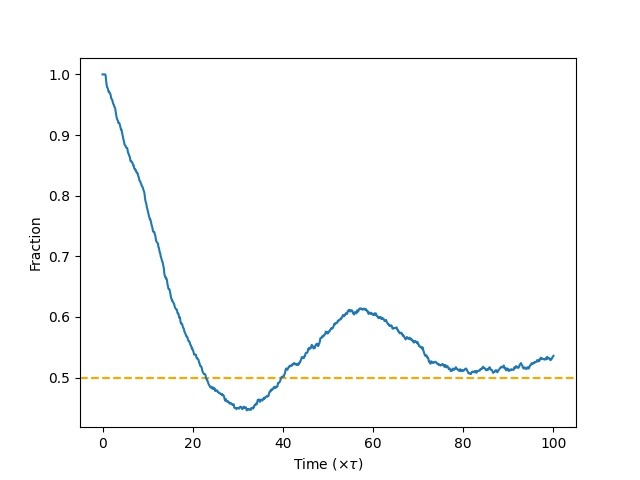
\includegraphics[width=.7\textwidth]{MD_90_1000_2_0.001_left_side_numbers.jpg}
  \caption{تغییرات نسبت ذرات موجود در نیمه‌ی چپ جعبه بر حسب زمان شبیه‌سازی برای $1000$ ذره‌ی آرگون در جعبه‌ای به طول $90$ و با سرعت اولیه‌ی $1.5$}
  \label{fig:1000_left_side}
\end{figure}


\subsection{دمای گاز}
رفتار دما کاملا مشابه با رفتار انرژی جنبشی است. تنها اسکیل آن‌ها متفاوت می‌باشد.
نمودار به دست آمده را در شکل
\ref{fig:1000_temperature}
می توان مشاهده نمود.
همان‌طور که دیده می‌شود دما در حدود زمان
$40$
به تعادل می رسد و حول آن نوسان می کند.
از آن‌جایی که تعداد ذرات ما کم است، دامنه‌ی این نوسانات به نسبت زیاد می‌باشد.
با میان‌گیری زمانی مقدار تعادلی آن برابر می‌شود با:
\begin{equation}
  \braket{T} = 1.309 \pm 0.001 \ (\times \epsilon / k_B) = 156.7 \pm 0.1 K
\end{equation}

\begin{figure}[h!]
	\centering
  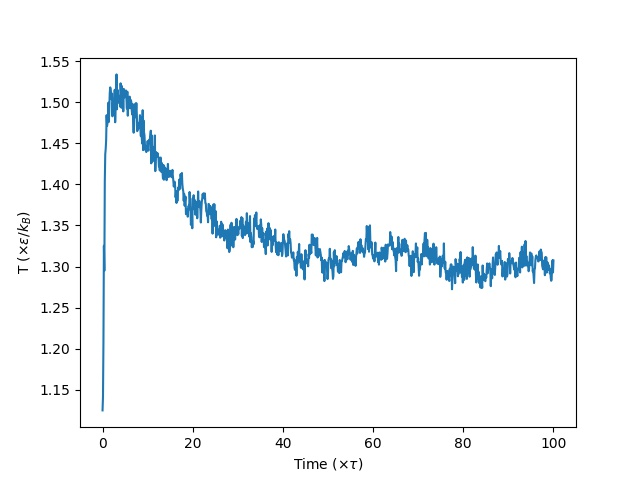
\includegraphics[width=.7\textwidth]{MD_90_1000_2_0.001_temperatures.jpg}
  \caption{تغییرات دما بر حسب زمان شبیه‌سازی برای $1000$ ذره‌ی آرگون در جعبه‌ای به طول $90$ و با سرعت اولیه‌ی $1.5$}
  \label{fig:1000_temperature}
\end{figure}


\subsection{فشار گاز}
نمودار به دست آمده را در شکل
\ref{fig:1000_pressure}
می توان مشاهده نمود.
همان‌طور که دیده می‌شود فشار در حدود زمان
$30$
به تعادل می رسد و حول آن نوسان می کند.
از آن‌جایی که تعداد ذرات ما کم است، دامنه‌ی این نوسانات به نسبت زیاد می‌باشد.
با میان‌گیری زمانی مقدار تعادلی آن برابر می‌شود با:
\begin{equation}
  \braket{P} = 0.164 \pm 0.001 \ (\times \epsilon / \sigma^2) = (2.3405 \pm 0.0001) \times 10^{-3} N/m
\end{equation}

\begin{figure}[h!]
	\centering
  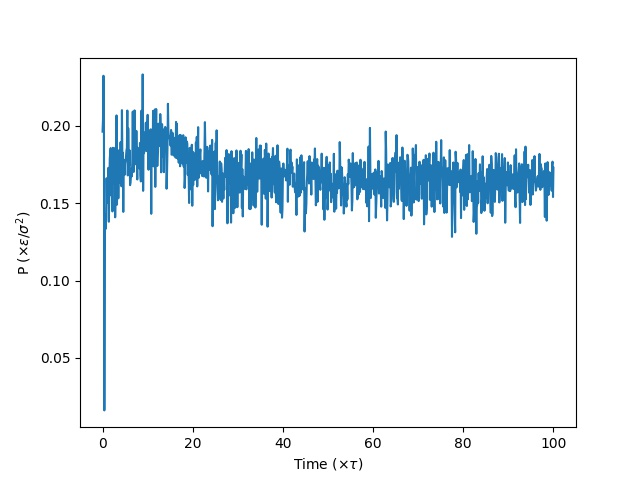
\includegraphics[width=.7\textwidth]{MD_90_1000_2_0.001_pressures.jpg}
  \caption{تغییرات فشار بر حسب زمان شبیه‌سازی برای $1000$ ذره‌ی آرگون در جعبه‌ای به طول $90$ و با سرعت اولیه‌ی $1.5$}
  \label{fig:1000_pressure}
\end{figure}


\subsection{خودهم‌بستگی سرعت‌ها و زمان واهلش}
زمان واهلش، زمان مشخصه‌ی تابع خود‌هم‌بستگی سرعت‌ها است.
این زمان در واقع به ما نشان می دهد که چقدر زمان باید بگذرد تا سرعت‌های سیستم مقادیر اولیه خود را فراموش کنند.
نمودار به دست آمده را در شکل
\ref{fig:1000_c_v}
می توان مشاهده نمود.
با توجه به نمودار به دست آمده، زمان واهلش برابر خواهد بود با:
\begin{equation}
  \tau = 1.8 (\times \tau)
\end{equation}

\begin{figure}[h!]
	\centering
  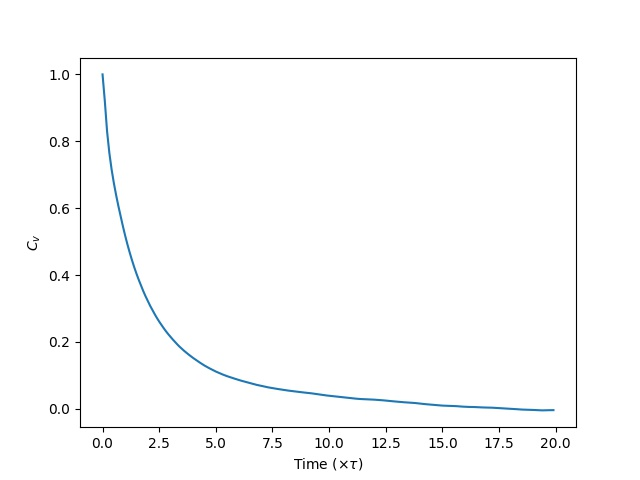
\includegraphics[width=.7\textwidth]{MD_90_1000_2_0.001_c_v.jpg}
  \caption{تابع خود‌هم‌بستگی سرعت‌ها برای $1000$ ذره‌ی آرگون در جعبه‌ای به طول $90$ و با سرعت اولیه‌ی $1.5$}
  \label{fig:1000_c_v}
\end{figure}

\end{document}
